\documentclass[11pt, a4paper, leqno]{article}
\usepackage{a4wide}
\usepackage[T1]{fontenc}
\usepackage[utf8]{inputenc}
\usepackage{float, afterpage, rotating, graphicx}
\usepackage{epstopdf}
\usepackage{longtable, booktabs, tabularx}
\usepackage{fancyvrb, moreverb, relsize}
\usepackage{eurosym, calc}
% \usepackage{chngcntr}
\usepackage{amsmath, amssymb, amsfonts, amsthm, bm}
\usepackage{caption}
\usepackage{mdwlist}
\usepackage{xfrac}
\usepackage{setspace}
\usepackage{xcolor}
\usepackage{subcaption}
\usepackage{minibox}
% \usepackage{pdf14} % Enable for Manuscriptcentral -- can't handle pdf 1.5
% \usepackage{endfloat} % Enable to move tables / figures to the end. Useful for some submissions.



\usepackage{natbib}
\bibliographystyle{rusnat}




\usepackage[unicode=true]{hyperref}
\hypersetup{
    colorlinks=true,
    linkcolor=black,
    anchorcolor=black,
    citecolor=black,
    filecolor=black,
    menucolor=black,
    runcolor=black,
    urlcolor=black
}


\widowpenalty=10000
\clubpenalty=10000

\setlength{\parskip}{1ex}
\setlength{\parindent}{0ex}
\setstretch{1.5}


\begin{document}

\title{Dating Structural Changes in Linear Regression Models - A \texttt{Python} implementation\thanks{Felipe Augusto Azuero Mutis, Rheinische Friedrich-Wilhelms-Universität Bonn. Email: \href{mailto:s6feazue@uni-bonn.de}{\nolinkurl{s6feazue [at] uni-bonn [dot] de}}.}}

\author{Felipe Augusto Azuero Mutis}

\date{
{\bf Preliminary -- please do not quote}
\\[1ex]
\today
}

\maketitle


\begin{abstract}
	This document presents an analysis of the \texttt{breakpoints} function programmed in \texttt{Python}, based on \texttt{R}'s \texttt{strucchange} package, whose objective is to obtain dating of the breakpoints in data that may have one or more structural changes in a linear model. The results obtained from the timing of the function are presented, as well as an implementation with data concerning the historical homicide rate in Colombia.
\end{abstract}
\clearpage

\section{The Model} % (fold)
\label{sec:model}

Consider the simple linear regression model with \textit{m} unknown breaks:
\begin{align} \label{eq:lm}
    y_t &= x'_{t}\beta_{j} + u_{t}  & (t &= T_{j-1}+1...+T_{j+1}, & j &= 1,...,m+1 )
\end{align}
The aim is to estimate the indexes $(T_{1},...,T_{m})$, where $T_{0} = 0$ and $T_{m+1} = T$ by minimizing the sum of residual squares of the equation \ref{eq:lm}.  To achieve this, an algorithm based on the principle of dynamic programming is used, as described in \cite{bai2003computation}.

% section model (end)

\section{The Code}
\label{sec:code}
To implement the approach discussed above, the \texttt{breakpoints} function was programmed in \texttt{Python}. To facilitate the workflow, the template of \citet{gaudecker2019templates} was used.  A visual representation of the directed acyclic graph of the project can be seen in figure \ref{fig:1}. \\

\begin{figure}[h]

    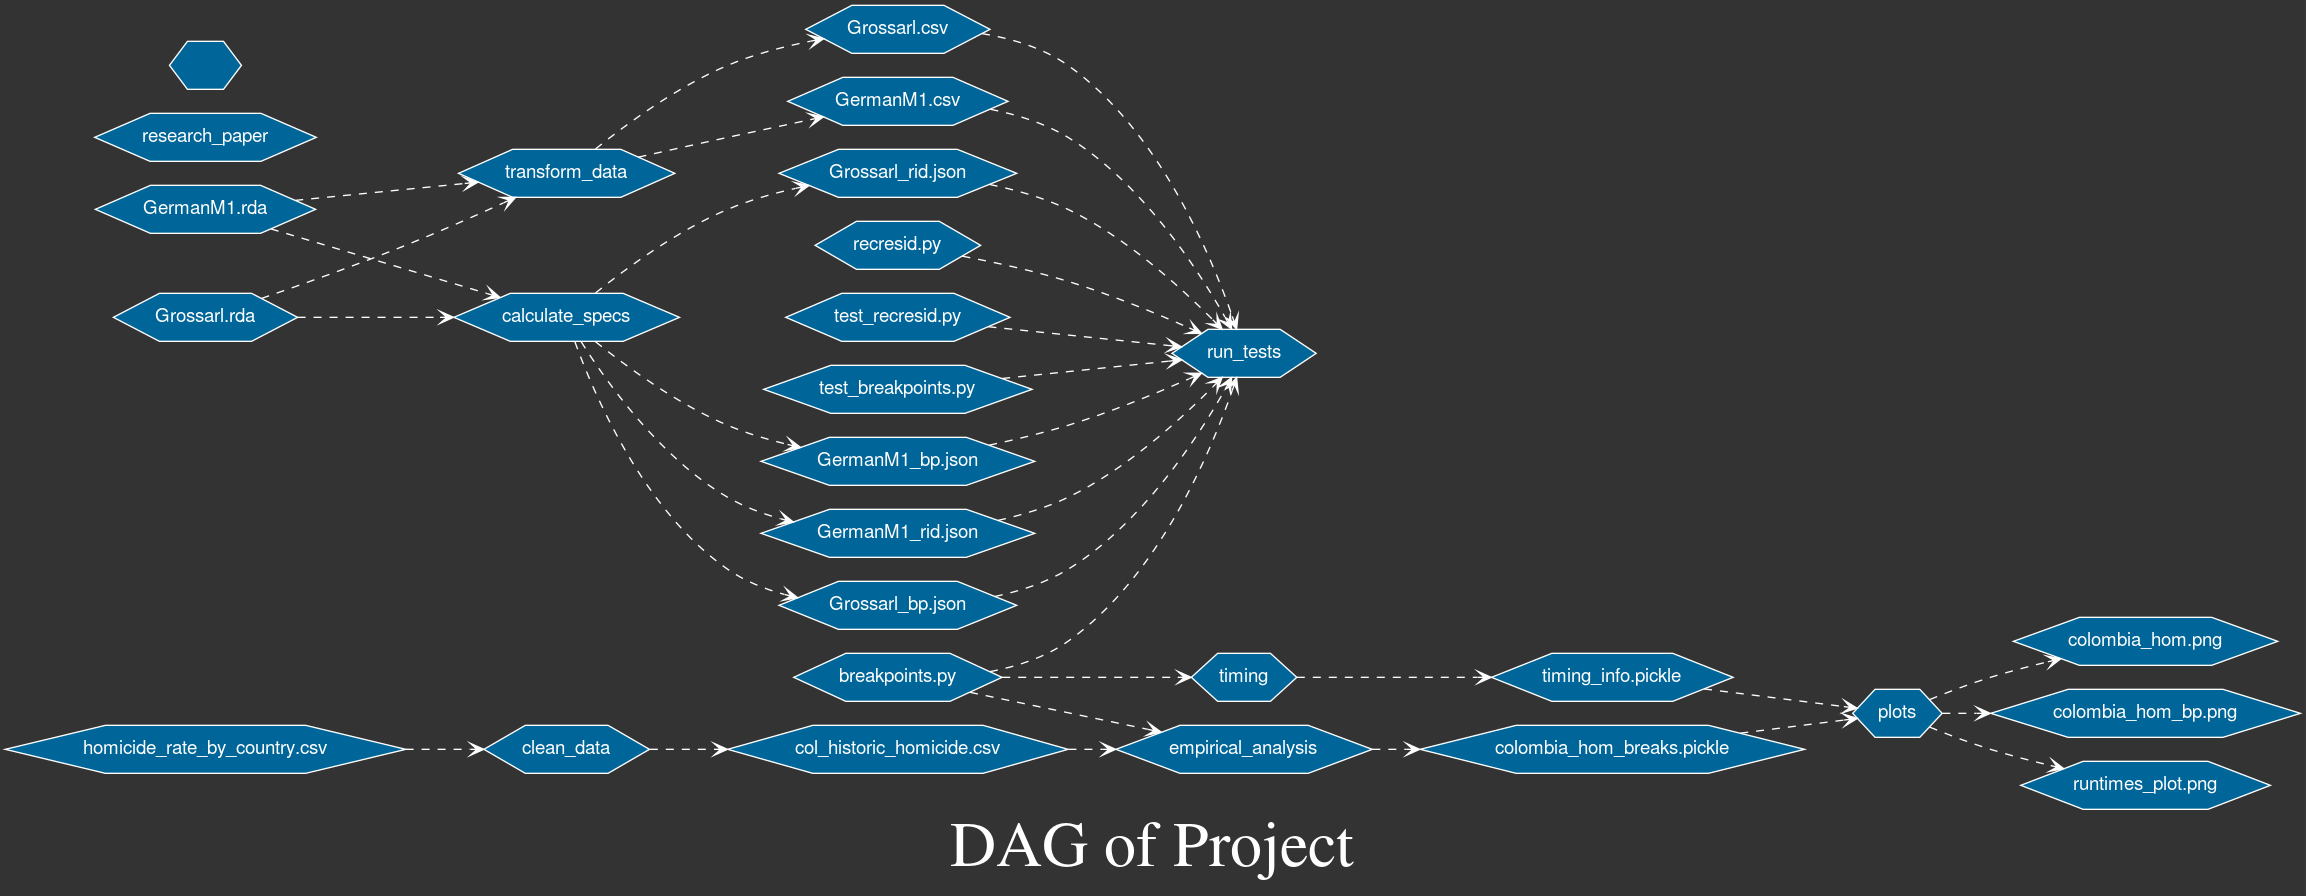
\includegraphics[width=\textwidth]{../../static/figures/dag}
    \caption{DAG of the Project}
    \label{fig:1}

\end{figure}

Since R has a package, \texttt{strucchange} (\citealt{zeileis2019strucchange}), which has the same goal as the one we are looking to achieve, the \texttt{breakpoints} code is largely based on one of the methods from the package.

\subsection{Timing the function}

To analyze the performance of the function, it was timed for different number of observations (Between $50$ and $500$ on steps of $25$), with $3$ explanatory variables.  The data used was on this process was seeded to contain 4 structural breaks. The timing of the function against the number of observations can be seen at figure \ref{fig:2}.

\begin{figure}[h]

    \includegraphics[width=\textwidth]{../../out/figures/runtimes_plot}
    \caption{Timing of the function.}
    \label{fig:2}

\end{figure}

% section code (end)

\section{Empirical Application}
\label{sec:empirical}

With the data obtained from the \cite{world2017homicides}, a small empirical application was conducted. Structural changes were sought in Colombia's homicide rate between 1990 and 2017. A view of the plotted data can be view in figure \ref{fig:3}.

\begin{figure}[ht]
    \centering
    \includegraphics[width=0.75\textwidth]{../../out/figures/colombia_hom.png}
    \caption{Homicide Rate in Colombia per Year.}
    \label{fig:3}

\end{figure}

There were 6 breakpoints found corresponding to the years 1995, 2000, 2003, 2005, 2008, 2014.  The results can be seen in the figure \ref{fig:4}.



\begin{figure}[ht]
    \centering
    \includegraphics[width=0.75\textwidth]{../../out/figures/colombia_hom_bp.png}
    \caption{Homicide Rate in Colombia per Year.}
    \label{fig:4}

\end{figure}

% section empirical (end)
\section{Conclusion}
\label{sec:conclusion}
Although the function seems to ``work'' on the desired task, further work is needed.  Testing with different number of independent variables and observations should be done. The code can also be cleaned to be more readable, more easy to work on, and more optimized.
\\
Still, the \texttt{breakpoints} function, here analyzed, facilitates finding structural changes in linear regressions in a non-exogenous way and can be used in diverse applications.
% section conclusion (end)

\newpage

\bibliography{refs}


% The chngctr package is needed for the following lines.
% \counterwithin{table}{section}
% \counterwithin{figure}{section}

\end{document}
